\chapter{An attempt at Learning Decision Tree Policies with Reinforcement Learning}
\section{Grid Worlds}
\subsection{MDP}
We consider a 2×2 grid world Markov Decision Process (MDP) defined as follows:
\begin{itemize}
    \item \textbf{States}: Four cells labeled $S_0$, $S_1$, $S_2$, and $G$ (goal state) arranged in a 2×2 grid.
    \item \textbf{Actions}: At each state, the agent can move right ($\rightarrow$) or down ($\downarrow$) up ($\uparrow$) or left ($\leftarrow$).
    \item \textbf{Transitions}: Movements are deterministic, following the direction of the chosen action. Actions that would lead outside the grid leave the agent in the same state.
    \item \textbf{Rewards}: All transitions yield a reward of 0, except for any action taken from the goal state $G$, which yields a reward of 1.
    \item \textbf{Objective}: Maximize the expected discounted cumulative reward.
\end{itemize}

\begin{figure}[ht]
\centering
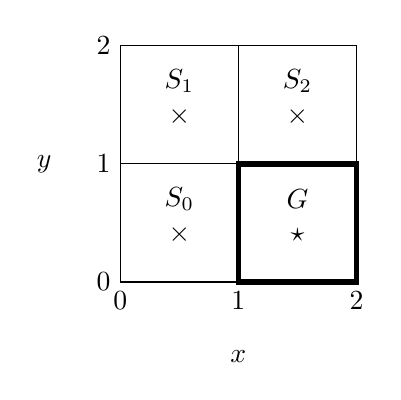
\begin{tikzpicture}[scale=1.5]
    % Draw the grid cells
    \draw (0,0) grid (2,2);
    
    % Add ticks on axes
    \foreach \x in {0,1,2}
        \node[below] at (\x,0) {$\x$};
    \foreach \y in {0,1,2}
        \node[left] at (0,\y) {$\y$};
    
    \node[left] at (-0.5, 1) {$y$};
    \node[below] at (1, -0.5) {$x$};
    
    % Label cells
    \node at (0.5,0.7) {$S_0$};
    \node at (0.5,0.4) {$\times$};

    \node at (0.5,1.7) {$S_1$};
    \node at (0.5,1.4) {$\times$};

    \node at (1.5,1.7) {$S_2$};
    \node at (1.5,1.4) {$\times$};

    
    % Goal state in bottom right with double border
    \draw[line width=2pt] (1,0) rectangle (2,1);
    \node at (1.5,0.7) {$G$};
    \node at (1.5,0.4) {$\star$};

    
\end{tikzpicture}
\caption{The 2×2 grid world environment with states $S_0$, $S_1$, $S_2$, and goal state $G$.}\label{fig:grid-world}
\end{figure}

\subsection{Solutions}

\begin{figure}[ht]
\centering
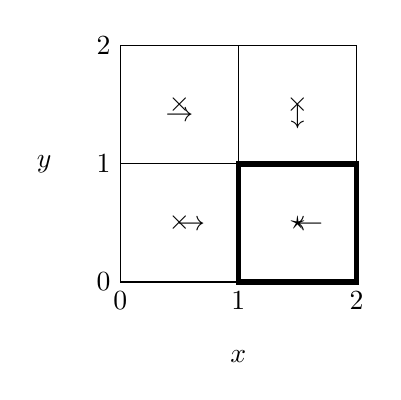
\begin{tikzpicture}[scale=1.5]
    % Draw the grid cells
    \draw (0,0) grid (2,2);
    
    % Add ticks on axes
    \foreach \x in {0,1,2}
        \node[below] at (\x,0) {$\x$};
    \foreach \y in {0,1,2}
        \node[left] at (0,\y) {$\y$};
    
    \node[left] at (-0.5, 1) {$y$};
    \node[below] at (1, -0.5) {$x$};
    
    % Label cells
    \node at (0.5,0.5) {$\times$};
    \node at (0.6,0.48) {$\rightarrow$};

    \node at (0.5,1.5) {$\times$};
    \node at (0.5,1.4) {$\rightarrow$};

    \node at (1.5,1.5) {$\times$};
    \node at (1.5,1.4) {$\downarrow$};
    
    % Goal state in bottom right with double border
    \draw[line width=2pt] (1,0) rectangle (2,1);
    \node at (1.5,0.5) {$\star$};
    \node at (1.6,0.48) {$\leftarrow$};

    
\end{tikzpicture}
\caption{An optimal tabular policy for the grid world.}\label{fig:optimal-policy}
\end{figure}


\subsection{Motivation}
The motivation is that for this simple grid world problem, indirect interpretable reinforcement learning algorithms can learn sub-optimal interpretability-performance trade-offs. E.g. we run Q-Learning to obtain an optimal tabular policy and then imitate this policy with decision trees with varying number of leaves. 

\begin{figure}[htbp]
    \centering
    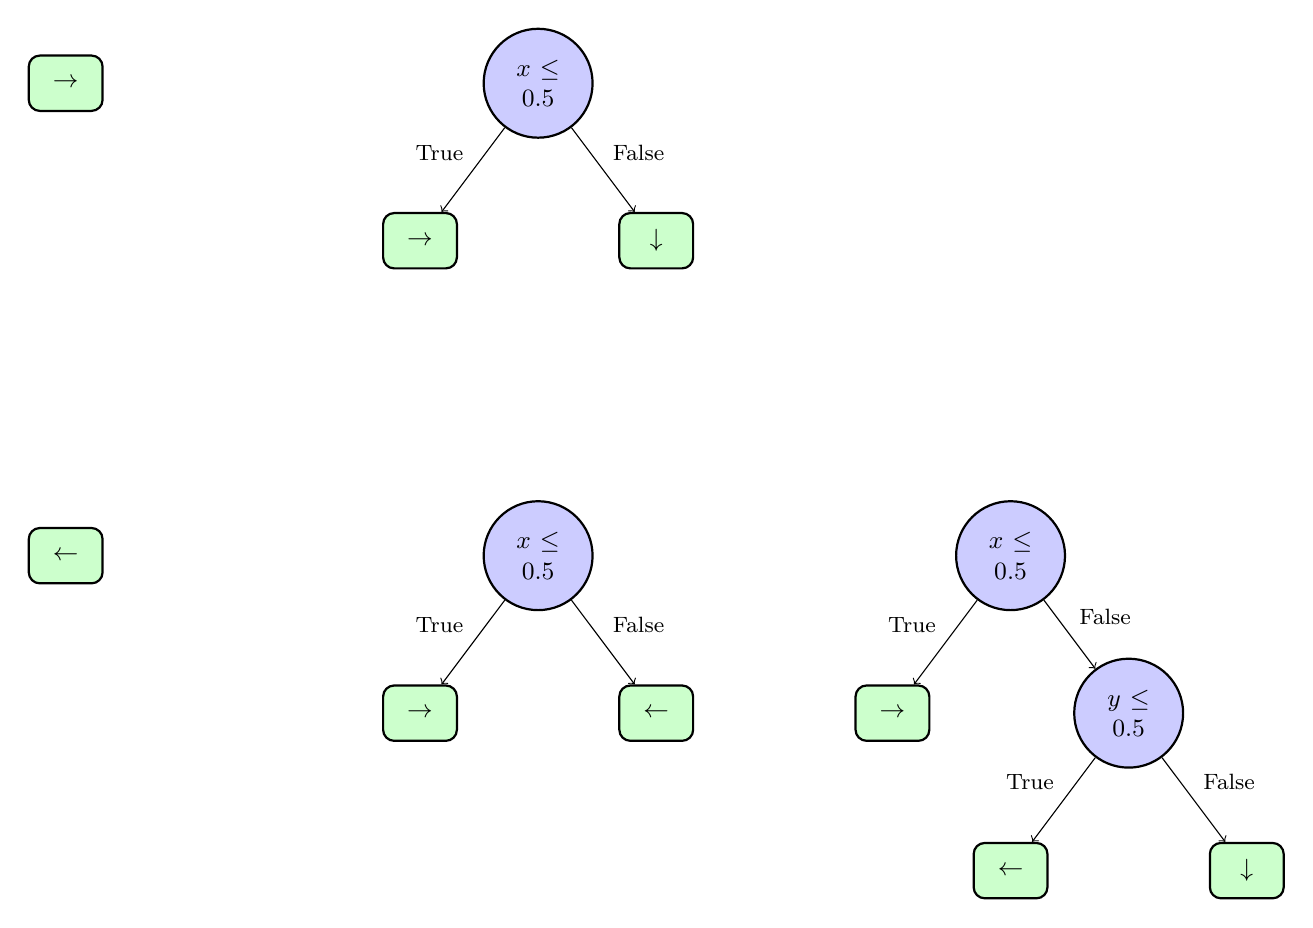
\begin{tikzpicture}[
        scale=1.0,
        decision/.style={circle, draw, thick, fill=blue!20, text width=2.5em, text centered, minimum height=2.5em, font=\small},
        leaf/.style={rectangle, draw, thick, fill=green!20, text width=2em, text centered, rounded corners, minimum height=2em, font=\small},
        edge_label/.style={font=\footnotesize, midway}
    ]
        % Tree 1: Move Right
        \node[leaf] (tree1) at (0,0) {$\rightarrow$};

        % Tree 3: if x <= 0.5 move right else move down
        \node[decision] (tree3_root) at (6,0) {$x \leq 0.5$};
        \node[leaf] (tree3_right) at (4.5,-2) {$\rightarrow$};
        \node[leaf] (tree3_down) at (7.5,-2) {$\downarrow$};
        \draw[->] (tree3_root) -- (tree3_right) node[edge_label, above left] {True};
        \draw[->] (tree3_root) -- (tree3_down) node[edge_label, above right] {False};

        % Tree 2: Move Left
        \node[leaf] (tree2) at (0,-6) {$\leftarrow$};

        % Tree 4: if x <= 0.5 move right else move left
        \node[decision] (tree4_root) at (6,-6) {$x \leq 0.5$};
        \node[leaf] (tree4_right) at (4.5,-8) {$\rightarrow$};
        \node[leaf] (tree4_left) at (7.5,-8) {$\leftarrow$};
        \draw[->] (tree4_root) -- (tree4_right) node[edge_label, above left] {True};
        \draw[->] (tree4_root) -- (tree4_left) node[edge_label, above right] {False};

        % Tree 5: if x <= 0.5: move right elif y <= 0.5 move left else move down
        \node[decision] (tree5_root) at (12,-6) {$x \leq 0.5$};
        \node[leaf] (tree5_right) at (10.5,-8) {$\rightarrow$};
        \node[decision] (tree5_y) at (13.5,-8) {$y \leq 0.5$};
        \node[leaf] (tree5_left) at (12,-10) {$\leftarrow$};
        \node[leaf] (tree5_down) at (15,-10) {$\downarrow$};
        \draw[->] (tree5_root) -- (tree5_right) node[edge_label, above left] {True};
        \draw[->] (tree5_root) -- (tree5_y) node[edge_label, above right] {False};
        \draw[->] (tree5_y) -- (tree5_left) node[edge_label, above left] {True};
        \draw[->] (tree5_y) -- (tree5_down) node[edge_label, above right] {False};
    \end{tikzpicture}
    \caption{Examples of decision trees for different policies in the grid world. Each tree represents a different policy, from simple single-action policies to more complex conditional policies.}
    \label{fig:policy-trees}
\end{figure}

\begin{figure}
    \centering
    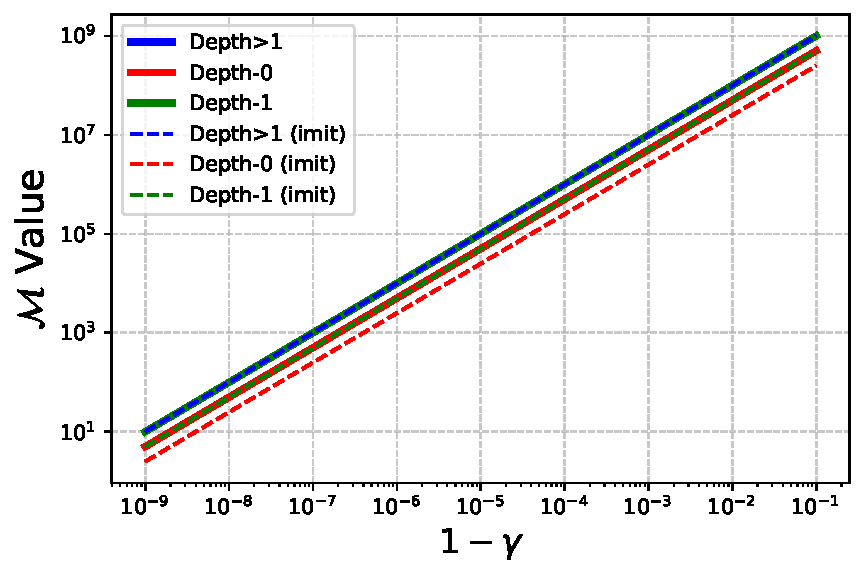
\includegraphics[width=1\textwidth]{images/images_part1/policy_values_comparison.pdf}
    \caption{Policy Values}\label{fig:policy-values}
\end{figure}


\section{Method}

As we saw above in Figure~\ref{fig:policy-values}, there exist policies whose interpretability-performance trade-offs can't be learn with indirect methods (cite).
IBMDPs are a direct method that should in theory, be able to learn the best trade-off.
However what we show next, is that it is very hard to make it work in practice.
Let us consider the IBMDP for the above grid world.
\paragraph{states:}
\paragraph{actions:}
\paragraph{transitions:}
\paragraph{rewards:}
\paragraph{objective:}


\section{Results}
\subsection{Dynamic Programming}
\begin{figure}[htbp]
    \centering
    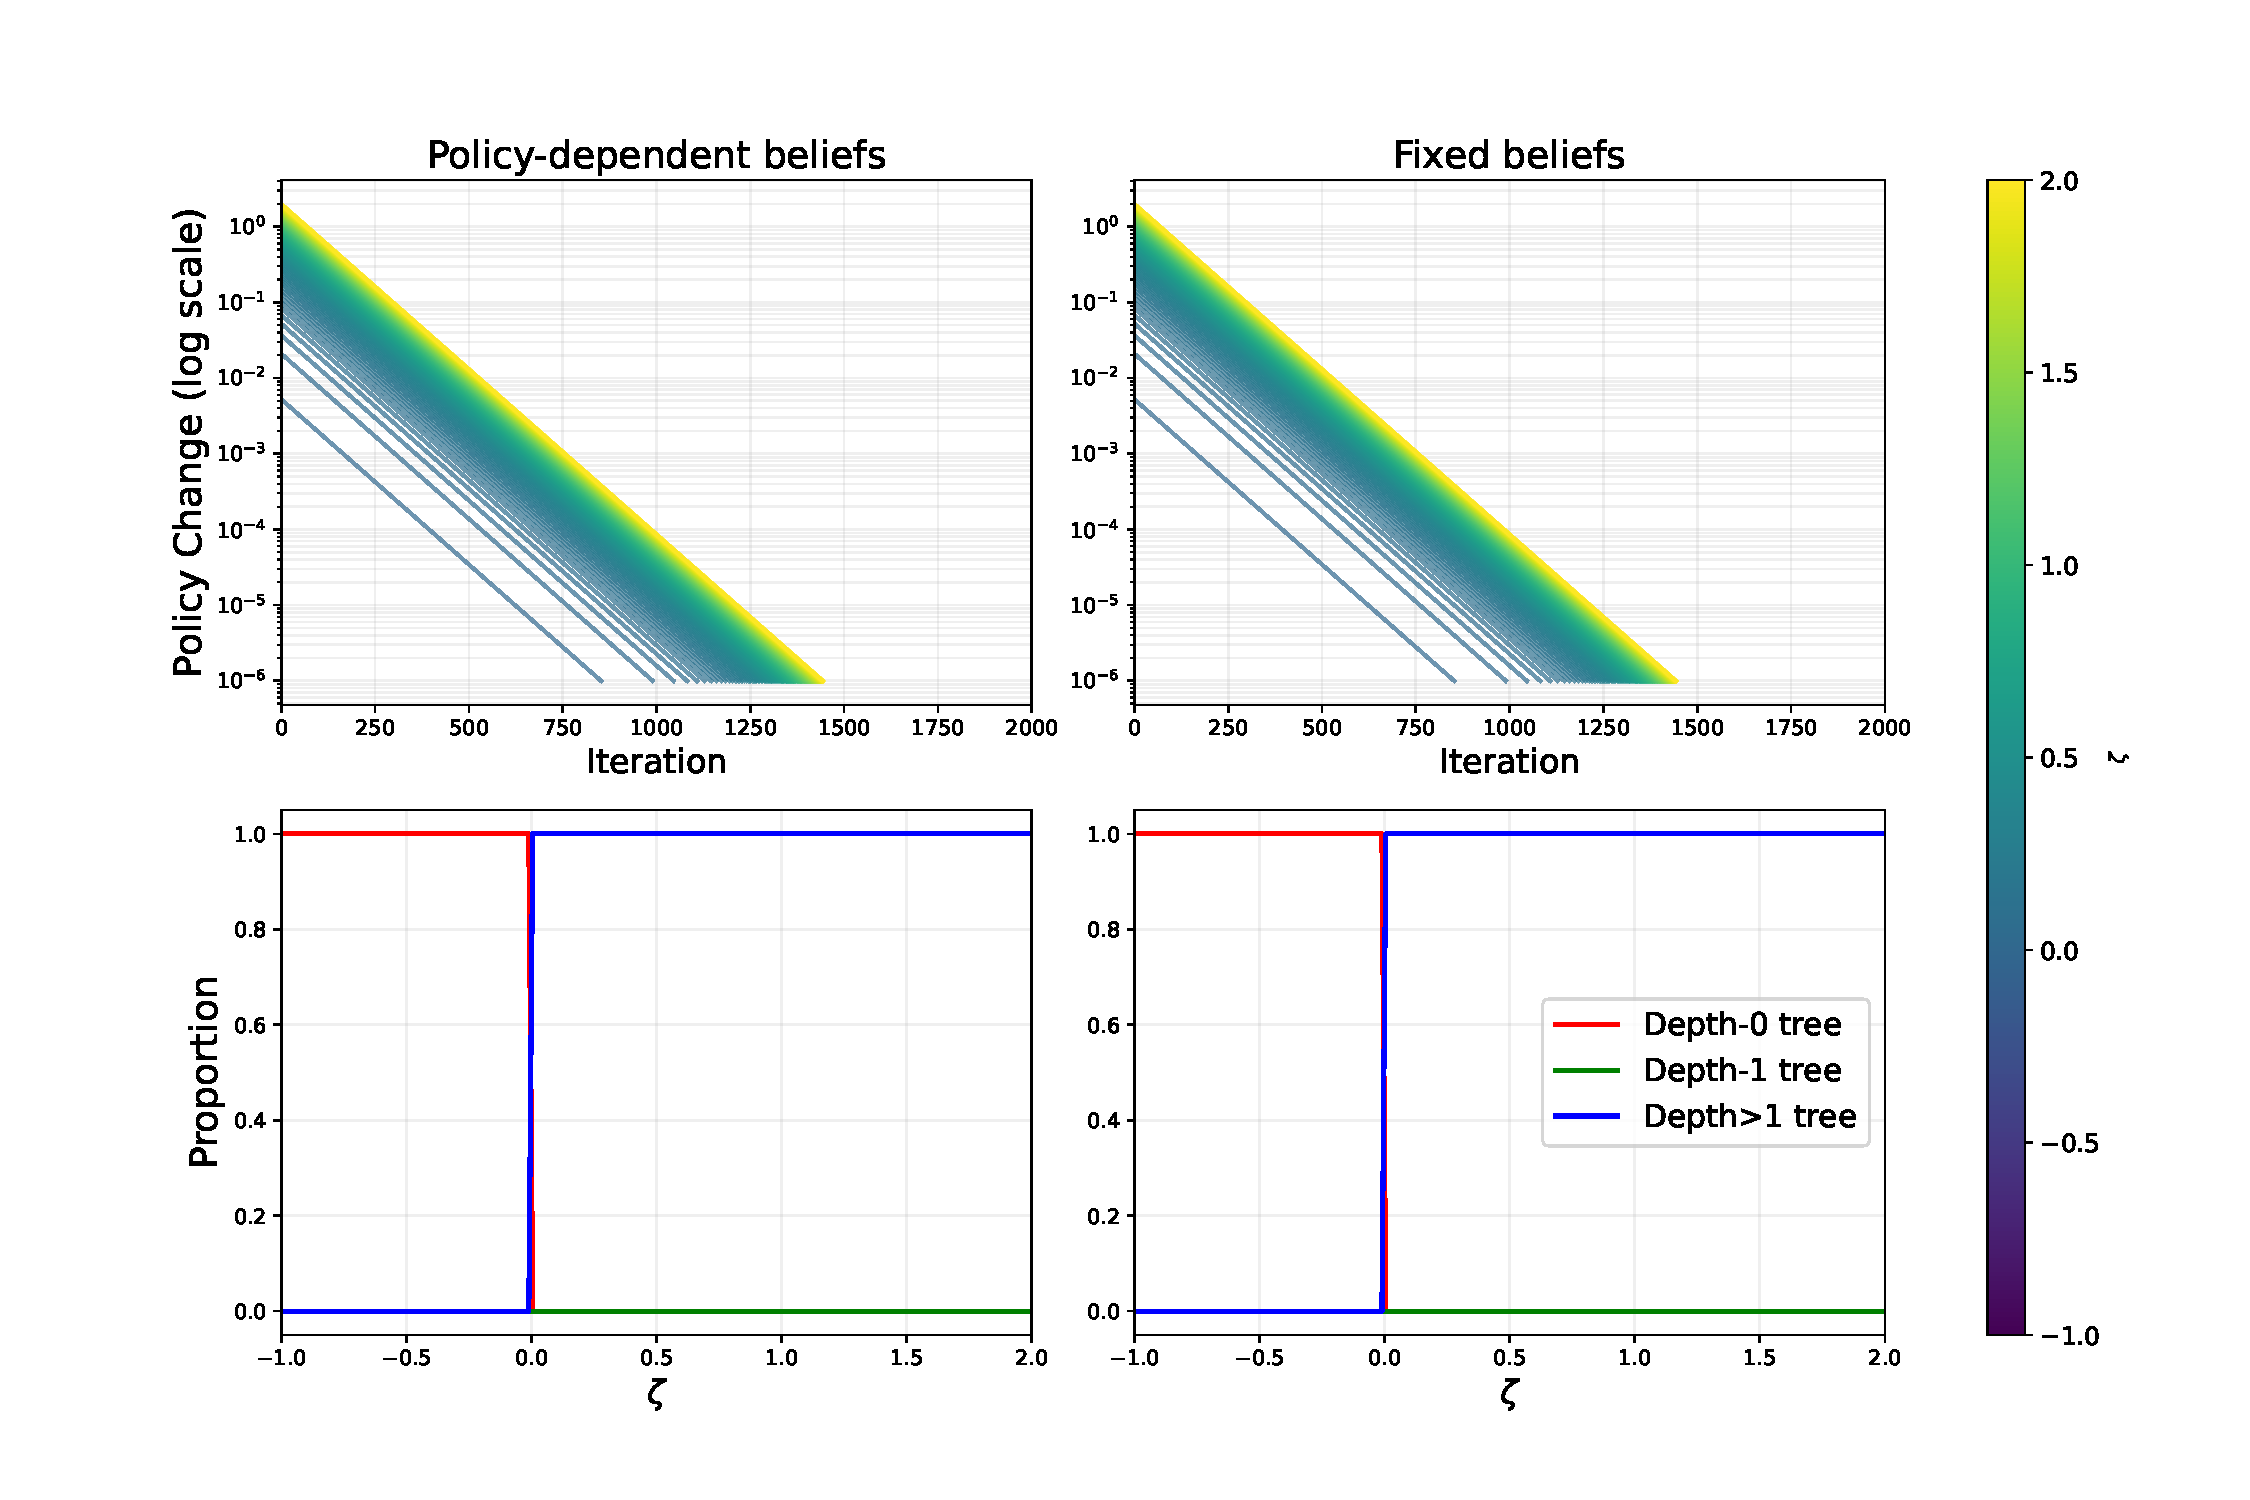
\includegraphics[width=1\textwidth]{images/images_part1/qiteration}
    \caption{Policy Values}\label{fig:dp}
\end{figure}
\subsection{Naive Reinforcement Learning}
\begin{figure}[htbp]
    \centering
    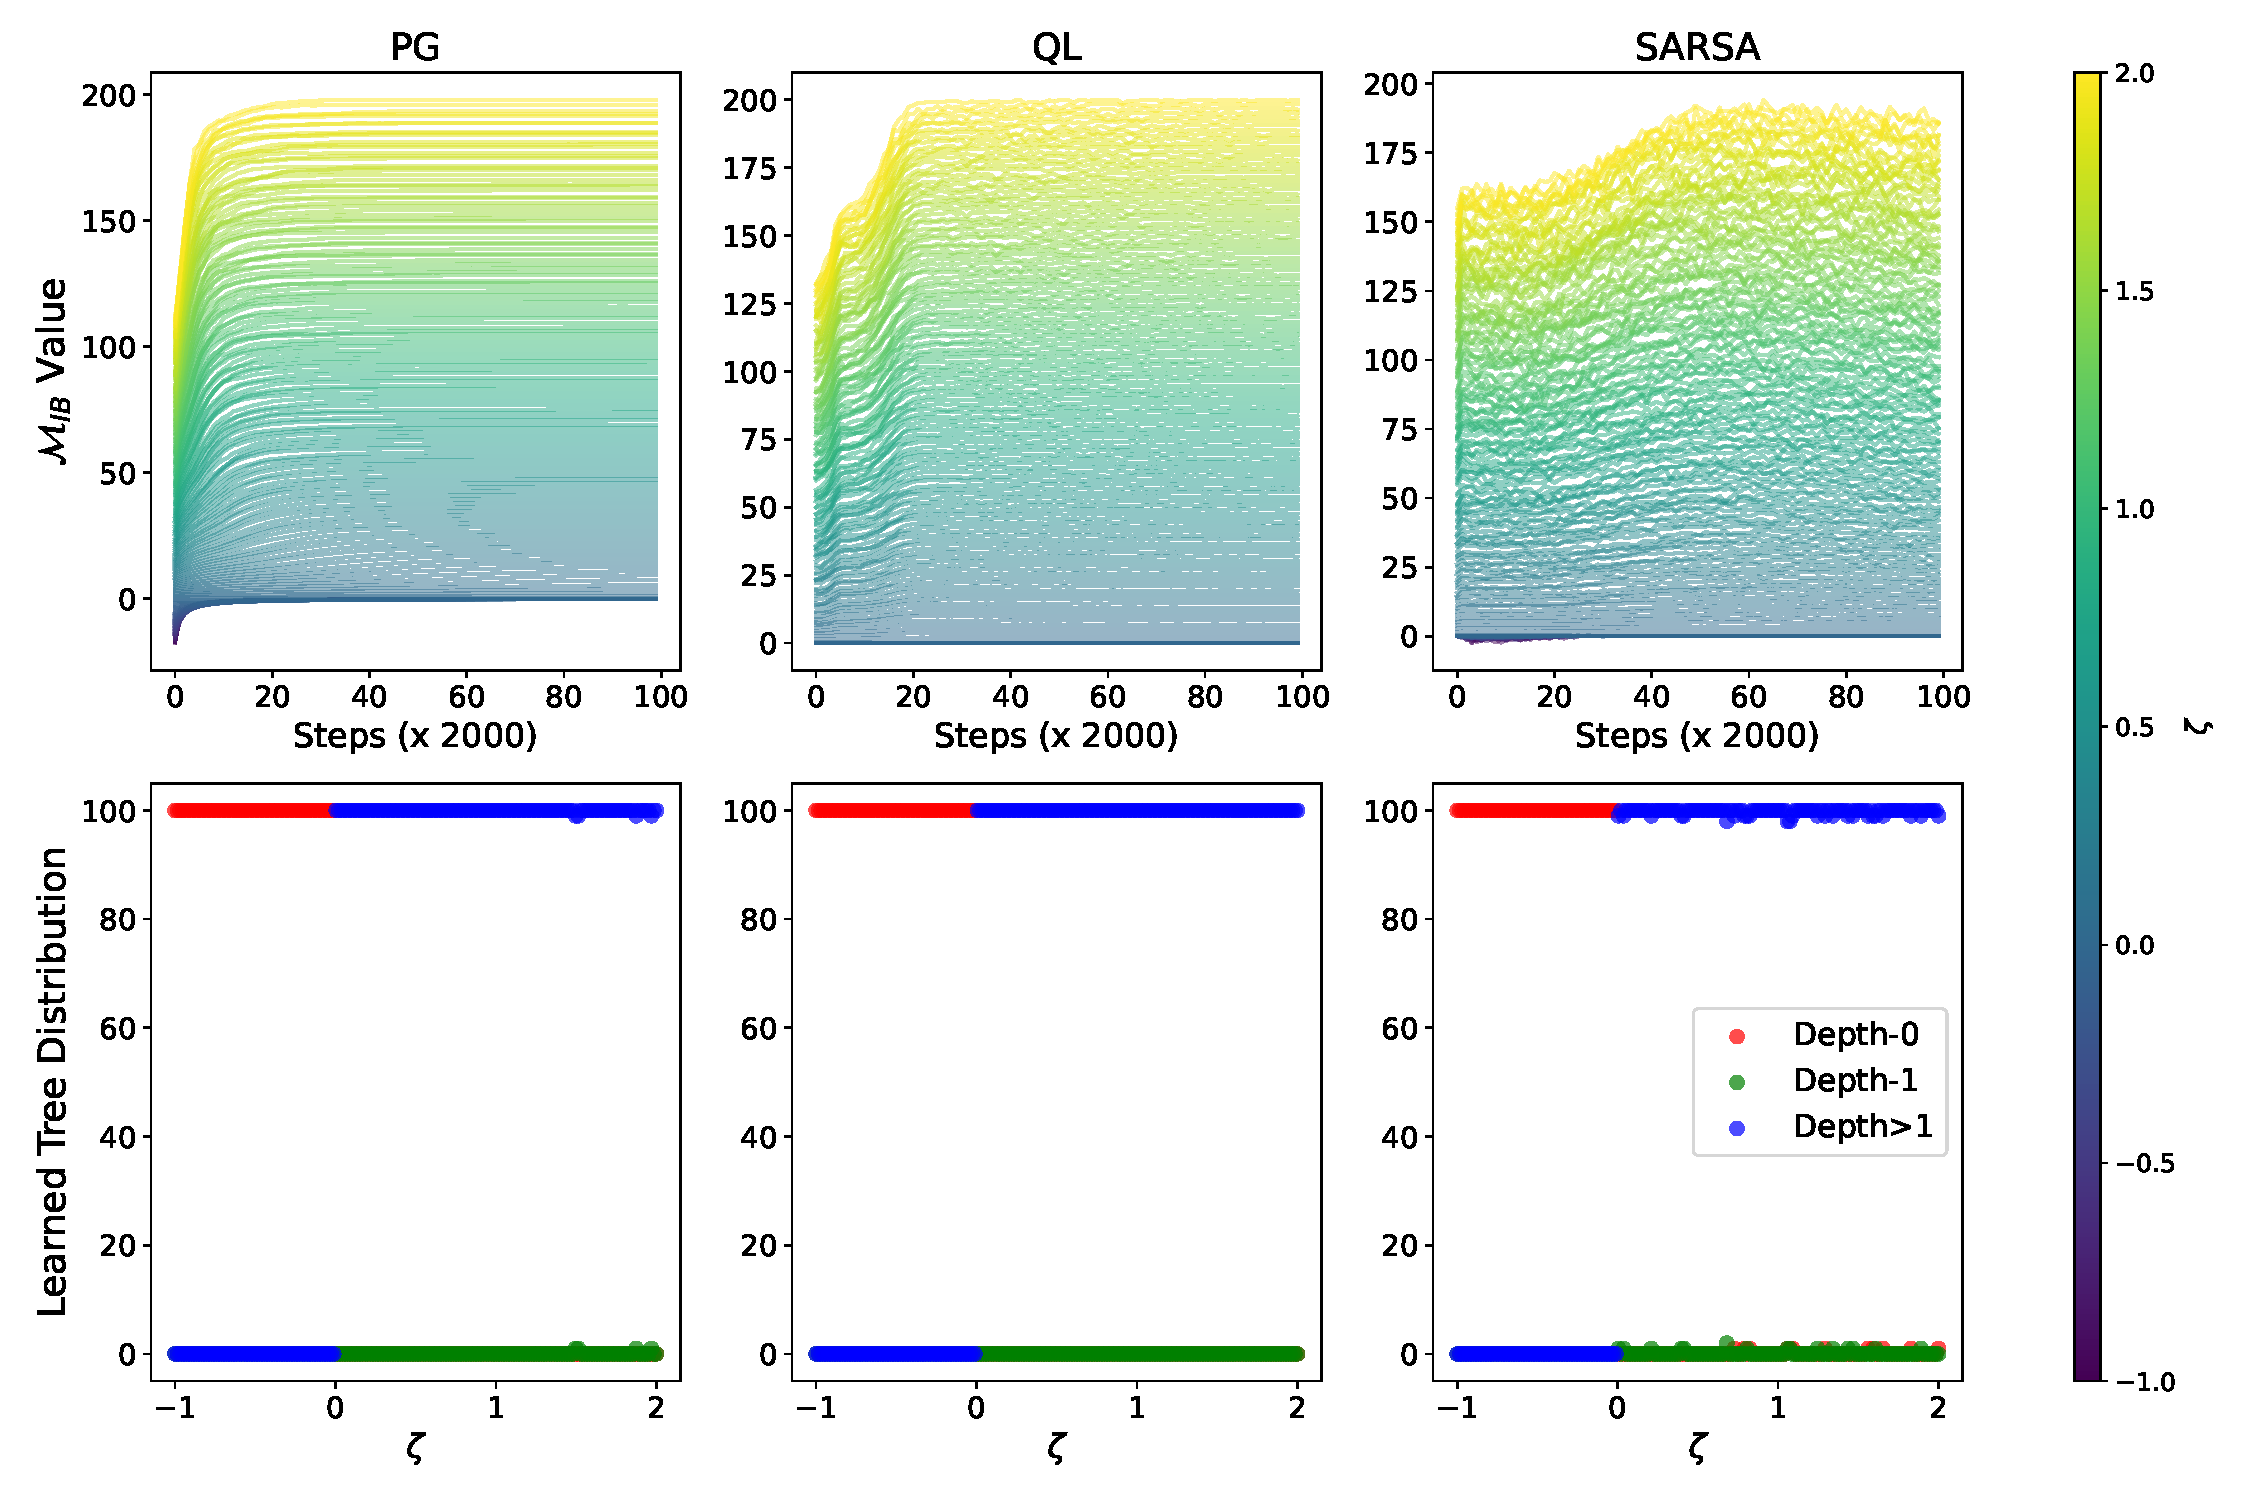
\includegraphics[width=1\textwidth]{images/images_part1/quick_plot_combined}
    \caption{Policy Values}\label{fig:naive-rl}
\end{figure}
We first start by plotting the learning curves of three classical RL algorithms described in the preliminaries. There was a series of work in the 1990's(cite) that studied the performances of RL algos when naively applied to he partially observable setting, i.e, naively setting $s\leftarrow o$.
The key observations are:
\begin{enumerate}
    \item The learning finishes, i.e, learning curves flatten after some iterations.
    \item There is a shift between the policies learned between the depth-0 tree and the depth>1 trees when $\zeta\geq0$.
\end{enumerate}
This is problematic because we know that \textit{theoretically}, for $0<\zeta<1$, the optimal policy for the IBMDP objective had depth $= 1$.
